\section{General}\label{sec:general3}
The construction of the planned models from chapter~\ref{ch:mechanics} required the use of 3D-printers, laser-cutters and CNC-machines.
As I did not have those heavy machines at home, I went to the FabLab Zurich\autocite{fablab} where I could use those machines.

\subsection{Shoot side manufacturing}\label{subsec:turn-side-manufacturing}
First I started with the move side and cut the holder, gear and gear rack from Plexiglas and printed the holder using the 3D-printers.
The first parts had a lot of issues regarding the spacing between the parts, they were either too loose or did not fit at all.
Then I printed the connecting part and mounted the inner part on the tube using a nail and a hole through the plastic and the aluminum tube and glowed the nail in place.

\subsection{Move side manufacturing}\label{subsec:move-side-manufacturing}
The other side turned out to be simpler, because there were only two parts: The holder and the small connector, which slides on the motor shaft and into the larger tube.
After having first used the wrong material for the 3D-printer, which resulted in a messy and unstable part, I successfully printed both parts.

\subsection{Camera holder}\label{subsec:camera-holder}
The camera holder also consists of two parts: the wooden base and the plastic holder.
I wanted to use wood for the base, as printing a larger rectangle would take a long time and would be a waste of material.
So I used a Computer numerical controlled (CNC) machine to cut out a hole where the 3D-printed part fits into nicely.
The camera holder required two attempts as the first time I did not make a larger hole for air to flow through to cool the camera.
The second model even had a hole for a small fan.
However, after \("\)carefully\("\) (touching it after letting it run for 10 min) measuring the cooling performance of the camera without a fan I came to the conclusion that the fan wasn't necessary.
\begin{figure}[H]
    \centering
    \begin{subfigure}{.5\textwidth}
        \centering
        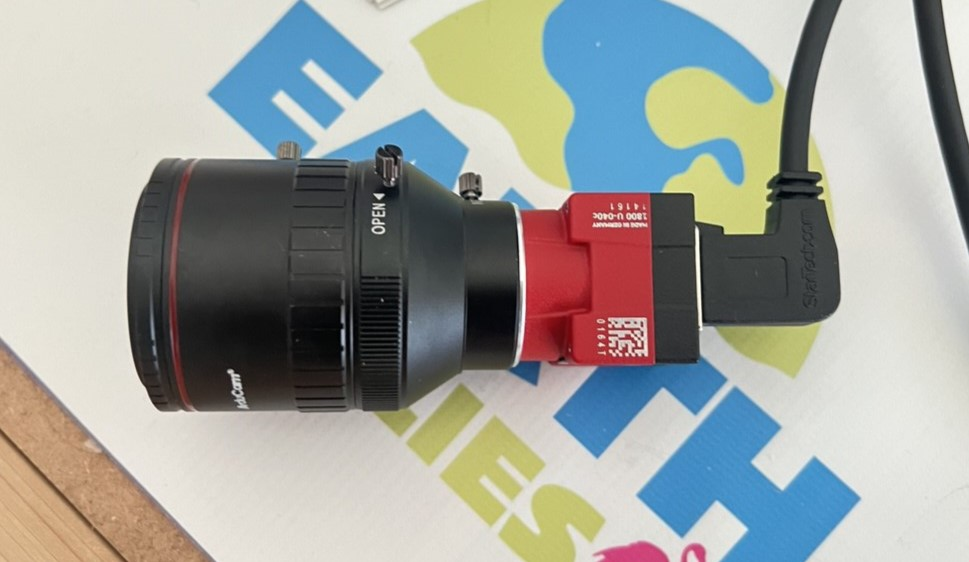
\includegraphics[width=.8\textwidth]{../photos/cam}
        \caption[cam]{Camera without holder}
        \label{fig:cam}
    \end{subfigure}%
    \begin{subfigure}{.5\textwidth}
        \centering
        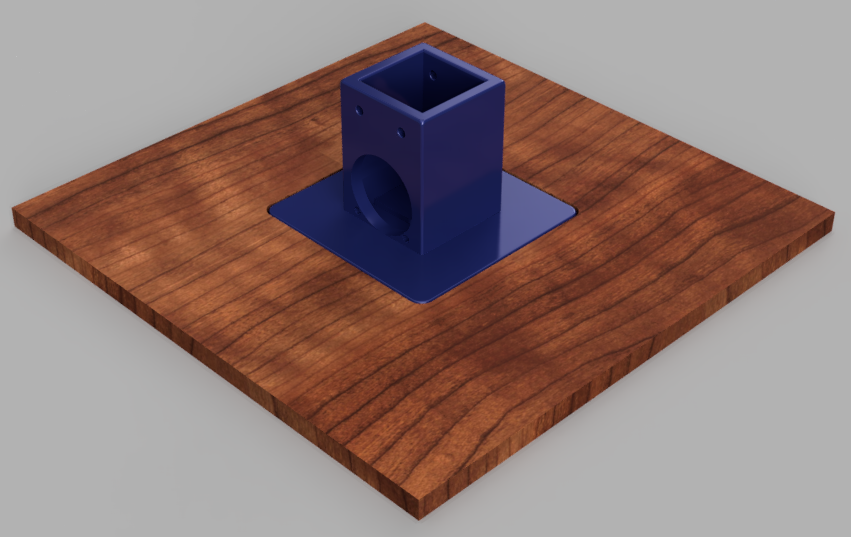
\includegraphics[width=.8\textwidth]{../photos/camholder_render}
        \caption[camholder]{Render of the camera holder}
        \label{fig:camholder_render}
    \end{subfigure}
    \caption{Undistorted example image}
    \label{fig:camholder}
\end{figure}